\documentclass[11pt]{article}
\usepackage{amssymb}
\usepackage{amsthm}
\usepackage{amsmath}
\usepackage{listings}
\usepackage{color}
\usepackage{graphicx}
\usepackage[margin=1.0in]{geometry}

\lstdefinestyle{matlab-style}{
language=Matlab,
basicstyle=\scriptsize\ttfamily,
tabsize=2,
rulecolor=,
language=matlab,
basicstyle=\scriptsize,
aboveskip={1.5\baselineskip},
columns=fullflexible,
showstringspaces=false,
extendedchars=true,
breaklines=true,
prebreak = \raisebox{0ex}[0ex][0ex]{\ensuremath{\hookleftarrow}},
frame=single,
showtabs=false,
showspaces=false,
showstringspaces=false,
identifierstyle=\ttfamily,
keywordstyle=\color[rgb]{0,0,1},
commentstyle=\color[rgb]{0.133,0.545,0.133},
stringstyle=\color[rgb]{0.627,0.126,0.941},
keepspaces=true,
numbers=left,
numbersep=5pt,
numberstyle=\tiny\color[rgb]{0.5,0.5,0.5},
stepnumber=1
}

\newcommand{\bs}[1] {\boldsymbol{#1}}

\title{Design of an optimal wing spar\\MANE 6963 - Project 2}
\author{ID: 2168}
\date{}

\begin{document}

\maketitle
\tableofcontents
\newpage

\section{Executive summary}

\begin{figure}[hbt]
\centering
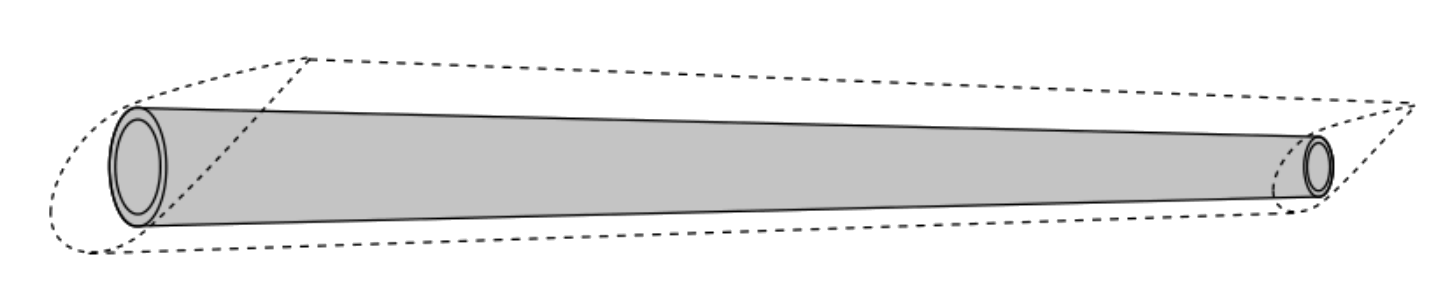
\includegraphics[width=0.6\textwidth]{spar}
\label{fig:spar}
\caption{Wing (dotted lines) and illustration of spar geometry}
\end{figure}

In this report, we investigate the optimal design of a
spar as the primary support for the wing of an aircraft.
Figure \ref{fig:spar} shows an illustration of the spar
that is to be designed. Our main objective is to minimize the
weight (and thus the mass) of the wing spar subject to
engineering operational assumptions about the aircraft,
engineering design assumptions, and aircraft
operational assumptions. These assumptions and
constraints are outlined below:

\subsection{Aircraft operational assumptions}

We assume that the total mass of the aircraft
is $m_{\text{plane}} = 500$ kg and that the weight
of the plane is equally supported by two wings.
Additionally, we assume that the plane is operating
at a $2.5$ g maneuver, where the span-wise force
distribution acting on the wing (and thus on the spar)
varies linearly, vanishing at the wing tip. The
distribution of this force per unit area $q(x)$
acting on the spar is shown in Figure \ref{fig:load}.

\begin{figure}[hbt]
\centering
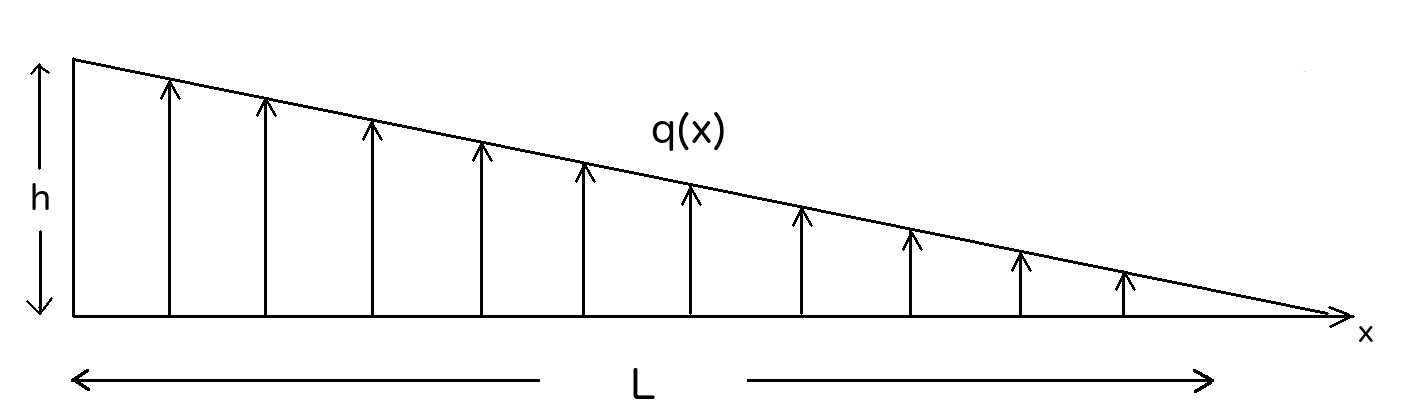
\includegraphics[width=0.6\textwidth]{load}
\caption{Load imposed on the wing}
\label{fig:load}
\end{figure}

\subsection{Engineering design assumptions}

We assume that the wing semi-span $L$ is $7.5$ m,
and that the spar supporting the wing will be made
of a composite fiber material. The material properties
of the composite are listed in Figure \ref{fig:materials}.
Additionally, we assume that the cross-section of
the spar in the $yz$ plane is a circular annulus,
as shown in Figure \ref{fig:annulus}.

\begin{figure}[hbt]
\centering
\begin{tabular}{ | l | r  |}
\hline
Material property & Value \\ \hline
Density $(\rho)$ & $1600$ km/m$^3$ \\ \hline
Young's modulus $(E)$ & $70$ GPa \\ \hline
Ultimate yield strength $(Y)$ & $600$ MPa \\ \hline
\end{tabular}
\caption{Material properties of the spar}
\label{fig:materials}
\end{figure}

\subsection{Engineering design constraints}

Due to material manufacturing restraints, we
assume that the inner radius of the spar at all
points $r_{\text{in}} \geq 1$ cm, and that the
inner and outer radii of the spar cannot be more
than $2.5$mm apart, i.e.
$r_{\text{out}} - r_{\text{in}} \geq 2.5$ mm.
Because the spar must remain within the wing, we
constrain the outer radius of the spar to be less
than or equal to $5$ cm, i.e. $r_{\text{out}} \leq 5$cm.
Finally, we stipulate that the normal stress at all
span-wise locations in the be less than the yield
strength, $\sigma \leq Y$, to maintain a safe design.

\begin{figure}[hbt]
\centering
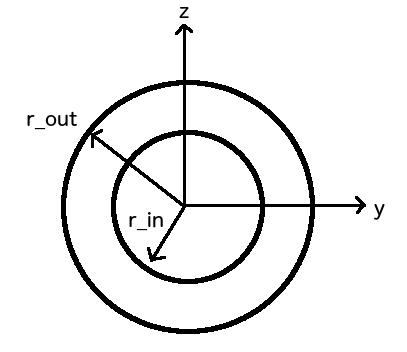
\includegraphics[width=0.3\textwidth]{annulus}
\caption{Annular cross-section of the spar geometry}
\label{fig:annulus}
\end{figure}

\subsection{Work done to achieve optimization goal}

To achieve our optimization goal given the stated constraints
we have:
\begin{itemize}
\item Determined a suitable geometry representation for the spar
\item Implemented 
\item Utilized a finite element analysis 
\end{itemize}

\section{Geometry representation}

\section{Analysis methods}

\section{Optimization problem statement}

\section{Optimization methods}

\section{Results}

\section{Conclusions}

\newpage

\section{Appendix: code listings}

\lstinputlisting[style=matlab-style,caption=CalcForce.m]{CalcForce.m}
\lstinputlisting[style=matlab-style,caption=CalcMoment.m]{CalcMoment.m}
\newpage
\lstinputlisting[style=matlab-style,caption=CalcMass.m]{CalcMass.m}
\lstinputlisting[style=matlab-style,caption=ConstraintLower.m]{ConstraintLower.m}
\newpage
\lstinputlisting[style=matlab-style,caption=ConstraintUpper.m]{ConstraintUpper.m}
\lstinputlisting[style=matlab-style,caption=ConstraintStress.m]{ConstraintStress.m}
\newpage
\lstinputlisting[style=matlab-style,caption=Obj.m]{Obj.m}
\lstinputlisting[style=matlab-style,caption=Plotter.m]{Plotter.m}
\newpage
\lstinputlisting[style=matlab-style,caption=Driver.m]{Driver.m}

\end{document}
